\section*{Introduction mathématique}
\addcontentsline{toc}{section}{Introduction mathématique}

Ce manuscrit se concentre sur des problèmes de Cauchy de la forme 
\begin{equation} \label{sec:intro:eq:u}
  \pa_t u^\eps = -\frac{1}{\eps}A u^\eps + f( u^\eps ),
  \qquad u^\eps(0) = u_0 
\end{equation}
où $t$ évolue dans l'intervalle $[0,1]$. On considère ce problème dans un Banach $(E, |\cdot|)$ de dimension finie $d >0$, avec $A : E \rightarrow E$ un opérateur linéaire et $f : E \rightarrow E$ un champ de vecteurs régulier. On se concentre sur le cas où~$A$ est diagonal avec des valeurs propres positives entières. Souvent, on séparera le problème entre le noyau et l'image de~$A$, pour obtenir un problème de la forme 
\begin{subequations} \label{sec:intro:eq:xz}
  \begin{empheq}[left=\left\lbrace, right=\right.]{align} &
    \pa_t x^\eps = a(x^\eps, z^\eps) , & &
    x^\eps(0) = x_0 , \vphantom{\frac11}\qquad\qquad
    \\ & 
    \pa_t z^\eps = -\frac{1}{\eps}\Lambda z^\eps + b(x^\eps, z^\eps) , & &
    z^\eps(0) = z_0 
  \end{empheq}
\end{subequations}
avec $u = \begin{pmatrix} x \\ z \end{pmatrix}$, $A = \begin{pmatrix} 0 & 0 \\ 0 & \Lambda \end{pmatrix}$ et $f = \begin{pmatrix} a \\ b \end{pmatrix}$. En général, on omettra l'exposant~$\eps$. Le lecteur peut supposer que, sauf mention contraire, toutes les variables dépendent de $\eps$. D'ailleurs, on peut supposer que le champ de vecteurs~$f$ évolue de manière régulière en fonction de~$\eps$ sans impacter les résultats. 

Dans cette section on décrit et illustre le comportement de la solution $(x^\eps, z^\eps)$ à travers deux exemples. En particulier, on énonce le théorème de variété centrale, qui décrit le comportement de la solution en temps long, et on présente rapidement une méthode pour calculer cette variété centrale. On introduit ensuite quelques hypothèses qui permettront de citer des résultats d'estimation numérique rigoureux dans la prochaine section. 


\subsection*{Quelques observations}
\addcontentsline{toc}{subsection}{Quelques observations}

Pour démarrer, considérons le problème jouet suivant
\begin{equation} \label{sec:intro:pb:z_sin}
    \pa_t z(t) = -\frac{1}{\eps}z(t) + \sin(t), 
    \qquad
    z(0) = 1, 
\end{equation}
qui peut être transformé en un problème de la forme~\eqref{sec:intro:eq:xz} en posant $x(t) = t$, soit $\pa_t x = 1,\ x(0) = 0$. Ce problème peut être obtenu à partir de 
\begin{equation*}
    \pa_t y(t) = -\frac{1}{\eps} \big( y(t) - \cos(t) \big), 
    \qquad
    y(0) = 0, 
\end{equation*}
en posant $z(t) = y(t) - \cos(t)$. C'est un problème de référence pour l'introduction aux systèmes raides: c'est le premier exemple présenté dans~\cite{hairer.1996.solving}. La solution exacte se calcule sans difficulté en intégrant $\pa_t \big[ e^{t/\eps} z(t) \big]$, ce qui donne 
\begin{equation} \label{sec:intro:sol:z_sin}
    z(t) = e^{-t/\eps} \left( 1 + \frac{\eps^2}{1+\eps^2} \right)
        + \frac{\eps}{1 + \eps^2} \big( \sin(t) - \eps \cos(t) \big) .
\end{equation}

On observe que la solution comporte deux parties de natures différentes, la phase transitoire (en $e^{-t/\eps}$) et la variété centrale (en $t$) de taille $\eps$. Ces deux phases apparaissent clairement sur la figure ci-dessous où on a tracé la solution et la variété centrale associée pour trois valeurs de~$\eps$. En effet, le temps d'atteinte de la variété semble proportionnel à~$\eps$ pour des petites valeurs. 
%
\begin{figure}[!ht]
    \centering
    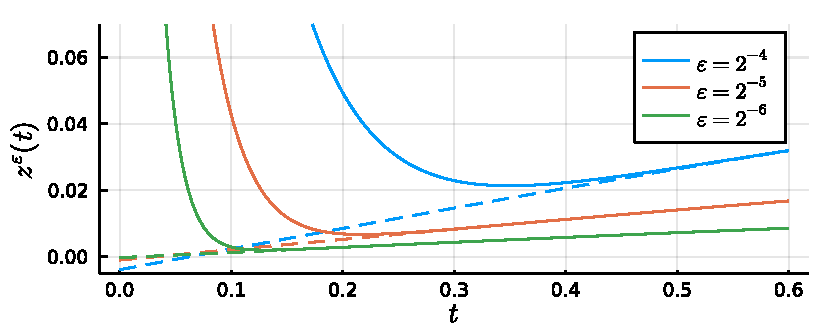
\includegraphics{./Presentation/z_sin.pdf}
    \caption{Comportement de la solution~\eqref{sec:intro:sol:z_sin} pour différentes valeurs de~$\eps$, avec chaque variété centrale associée en pointillés.}
\end{figure}

En fait, dans le cas d'un système de la forme~\eqref{sec:intro:eq:xz}, la dynamique en temps long est déterminé entièrement par la variable $x$. Il y a une réduction de dimension, qui est traduite dans le théorème de variété centrale. 
\begin{FRtheorem*}[Variété centrale, \cite{carr.1982.applications}]
    En supposant que le champ $f$ est dans $C^\infty(E)$ et que la donnée initiale $u_0 \in E$ du problème~\eqref{sec:intro:eq:u} est bornée, il existe un temps final $T > 0$ et un paramètre limite $\eps_0$ tels que le problème~\eqref{sec:intro:eq:u} est bien posé sur $[0,T]$. En outre, il existe une application régulière $x \mapsto z = \eps h^\eps(x)$, un taux $\mu > 0$ et une constante $c > 0$ tels que pour tout $t \in [0,T]$, 
    \begin{equation*}
        \left| z(t) - \eps h^\eps\big( x(t) \big) \right|
        \leq c e^{-\mu t/\eps} .
    \end{equation*}
    En outre, quitte à modifier $c$, il existe une donnée initiale \enquote{de l'ombre} $x_0^\eps$ telle que 
    \begin{equation*}
        \big| x(t) - \varphi_t^\eps \big( x_0^\eps \big) \big| 
        \leq c \eps e^{-\mu t/\eps} , 
    \end{equation*}
    où $\varphi^\eps_t$ est le $t$-flot associé au champ de vecteurs $x \mapsto a\big(x, \eps h^\eps(x) \big)$. On appelle l'ensemble des $\big( x, \eps h^\eps(x) \big)$ la variété centrale, qui est stable et \enquote{attire} la solution. 
\end{FRtheorem*}

Par exemple dans le cas~\eqref{sec:intro:pb:z_sin}, le morphisme de variété centrale $\eps h^\eps$ est donné par 
\begin{equation} \label{sec:intro:eq:h_sin}
    h^\eps(x) 
    = \frac{1}{1 + \eps^2} \big( \sin(x) - \eps \cos(x) \big) .
\end{equation}
Il est impossible d'espérer calculer le morphisme de variété centrale explicitement en général. On peut néanmoins appliquer une méthode de point fixe en remarquant qu'en temps long, $z \approx \eps h^\eps(x)$, d'où 
\begin{equation*}
    \pa_t z \approx \eps \pa_x h^\eps(x) \cdot \pa_t x
    \approx \eps \pa_x h^\eps(x) \cdot a(x, \eps h^\eps(x)) . 
\end{equation*} Ainsi on peut poser $h\rk 0 = 0$ et itérer de manière explicite
\begin{equation} \label{sec:intro:eq:iter_h}
    \eps \pa_x h\rk n(x) \cdot a(x, \eps h\rk n (x)) 
    = - h\rk{n+1}(x) + b(x, \eps h\rk n (x)) .
\end{equation}
Le calcul de la donnée initiale de l'ombre $x^\eps_0$ n'est en revanche pas si simple. La calculer demande de faire des développements sur l'intégralité du système et demande un certain investissement. Dans~\cite{castella.2016.formal}, les auteurs font appel à des B-séries\footnote{
    Les B-séries sont des séries formelles qui décrivent les solutions d'EDO. Cet outil, souvent utilisé pour développer des schémas numériques, est présenté en détails dans~\cite[Chap.~III]{hairer.2006.geometric} ou de manière plus concise dans~\cite{chartier.2010.algebraic}. Malgré une apparence encombrante, les B-séries possédent une structure algébrique élégante basée sur des opérations sur les arbres.
} pour obtenir un modèle asymptotique sur l'intégralité du problème~\eqref{sec:intro:eq:u}, à partir duquel ils trouvent en particulier cette donnée initiale modifiée, mais les calculs sont bien plus compliqués que~\eqref{sec:intro:eq:iter_h}.

\begin{FRremark*}
    Le phénomène de donnée initiale de l'ombre n'est cependant pas visible sur cet exemple, puisque la variable $x$ ne dépend pas de la dynamique sur $z$ (pour rappel, on a $x(t) = t$). L'interdépendance entre $x$ et $z$ apparaîtra dans le cas test de la section suivante.
\end{FRremark*}

On remarque deux caractéristiques importantes de la méthode d'approximation de $h^\eps$: elle nécessite de calculer une dérivée, ce qui demande du calcul symbolique potentiellement coûteux, et la convergence de la méthode n'est pas assurée. Même dans l'exemple jouet~\eqref{sec:intro:pb:z_sin}, cette méthode génère
\begin{equation*}
    h\rk{n}(x) = R_n(\eps) \sin(x) + \eps R_{n-1}(\eps) \cos(x) 
\end{equation*}
avec $R_n(\eps) = \sum_{k = 0}^{\left\lfloor n/2 \right\rfloor} \eps^{2k}$ et par convention $R_{-1} = 0$. En d'autres termes, on construit le développement en série entière en $\eps$ de la partie lente dans~\eqref{sec:intro:sol:z_sin}, i.e. $h\rk 1(x) = \sin(x)$, $h\rk 2 (x) = \sin(x) + \eps \cos(x)$ etc. Ainsi, le développement n'est convergent que pour $\eps < 1$, alors que la solution $z(t)$ converge vers la variété $\eps h^\eps(t)$ définie par~\eqref{sec:intro:eq:h_sin} pour tout $\eps > 0$. 
%
Cette limitation apparaîtra couramment au cours de ce manuscrit sous le format plus contraignant
\begin{equation*}
    \eps \leq \frac{\eps_0}{n+1} ,
\end{equation*}
qu'on peut remarquer par exemple avec $b(x,z) = (1+x)^{-1}$ dont la taille des dérivées évolue de manière factorielle avec l'ordre de dérivation. 




\subsection*{Définitions et hypothèses}
\addcontentsline{toc}{subsection}{Définitions et hypothèses}

% \todo[inline]{Rendre cette section plus fluide, les hypothèses sont parachutées}

On considère le problème~\eqref{sec:intro:eq:u} en dimension finie~$d$, et on suppose que la donnée initiale~$u_0$ appartient à un ensemble~$\mathcal{U}_0$ bien choisi de sorte qu'en tout temps, la solution appartient à un ensemble borné~$\mathcal{K}$ de la forme
\begin{equation*}
    \mathcal{K} := \left\{ \among{x}{z} \in E,\ \mathrm{s.t.}\ x \in \mathcal{K}_x, |z| \leq \rho  \right\} 
\end{equation*}
avec $\mathcal{K}_x$ borné et $\rho > 0$. Grâce au théorème de variété centrale, ces hypothèses peuvent être considérées valides pour tout $\eps \in (0, \eps_0]$ pour un certain $\eps_0 > 0$ fixé. 

En outre, on suppose que le champ de vecteurs $u \mapsto f(u)$ est de classe $C^\infty$ sur $\mathcal{K}_R$ pour un certain rayon $R > 0$, où
\begin{equation*}
    \mathcal{K}_R = \left\lbrace u \in \setR^d,\ d(u, \mathcal{K}) \leq R \right\rbrace 
\end{equation*} 
avec $d(u, \mathcal{K}) = \inf_{v \in \mathcal{K}} |u-v|$ la distance de $u$ à $\mathcal{K}$. Cette hypothèse permet d'assurer que les méthodes numériques se comportent bien au voisinage de la solution, sans nécessiter d'être exact pour autant. 